\chapter{System Design}

In this chapter, we want to present our system design. We will state the system requirements and our design choices. Finally, we will explain our system architecture. 

\section{System Requirements}
Before we can begin to design our system, we first need to define the requirements. Our goal is to capture data in a fully temporally aware manner and with organic controls. We specify the following requirements:

\begin{enumerate}
    \item \emph{Integration of Temporal Patterns} Our system should be able to encode timestamp information from the data.
    
    \item \emph{Online Training} Our system should adapt to new data in real-time. 
    
    \item \emph{Meta optimization} Our system should hybridize the different models with organic controls for optimal performance. 
\end{enumerate}


\section{Design Choices}
To fulfill the requirements, we introduce the following design choices:

\begin{enumerate}
    \item The datasets we use contain timestamps for every time a user interacted with an item. Since the BERT transformer processes all items in a sequence in parallel, it needs to encode the positional information. We extend the BERT encoder to encode the timestamp of each item in the sequence. Timestamps (in seconds since a fixed starting point) are transformed into vectors and added to the item encodings~\cite{mou2019t}. Additionally, we modify the BERT attention mechanism to focus more on events that occur within a short period and less on those with a large time gap.  
    
    % D.
    % (in seconds since a fixed starting point)
    
    \item We train our system with new data continuously. To do this efficiently, we first specify a dynamic window size based on the amount of new data being generated. At the end of each window, we train our system~\cite{misra1982finding,fan2000summary}. The embedding of sequences containing new items is postponed until the window boundary where we can afford to use more resources.
    
    \item We use a stacking hybridization approach with the help of regression~\cite{lee2021sunrise}. Our system adapts the weighting of models based on global prediction accuracy. Models can be added and removed dynamically if needed. We monitor each model in the system individually and reset or retrain a particular model as soon as the accuracy of the predictions declines. The system can continue to make predictions while one of the models is training.
\end{enumerate}


\section{System Workflow}
In this section, we will present our system workflow. Our system can be divided into i) machine learning using BERT, ii) a model-based approach with Markov chains and iii) the hybridization logic that combines the models. 

\subsection{ML Flow}
We will now present our ML workflow. It is based on the BERT model but with several extensions and improvements. At first, we created a custom uniform input converter that accepts a variety of datasets in different formats and parses them. It extracts timestamps if available and adds them to the input. To make BERT time-aware, we had to modify the BERT embedding layer. Tokenized items $x_i$ from the sequence are combined with a positional vector $p_i$ and a vector representing the time $t_i$ as follows: 

\begin{equation}
\setlength{\jot}{25pt}
    \begin{aligned}
        e_i=(x_i, p_i, t_i)
    \end{aligned}
    \label{equation:modified_embedding}
\end{equation}

After including the timestamps into the item embeddings to create temporal embeddings, we modified the transformer layers of BERT, specifically the attention mechanism, so that it can learn from temporal patterns. The modified version puts more attention on items that a user interacts with within a short period. Consequently, during an active user session items are more strongly associated with each other. There is a weaker association to items after an idle user session. During the training, our model learns to predict items that are frequently associated with similar active user sessions.

To make BERT dynamic and able to process data in batches, we modified BERT's training mechanism. Ar first, we modified the tokenizer. The traditional BERT model uses a fixed-sized vocabulary. We instead implemented a dynamic tokenizer that continually looks for unknown items and extends the vocabulary or shrinks it if an item is no longer relevant. Additionally, we introduced real-time training. We specify a window with dynamic size. We monitor the sequences for new items. Sequences with new items are added to the window. The embedding is postponed until the window boundary is reached. The size of the window is extended or reduced based on the available resources and workload.

Our model contains various hyperparameters that need to be fine-tuned.
We need to optimize the number of multi-attention heads, the maximum sequence length, and the number of items to mask in a sequence during training. Additionally, we need to optimize the duplication factor. We can duplicate sequences and mask different items each time for more training data when resources are available. All hyperparameters get passed to our automated meta-learning logic. 

% D.
% I'd rather try to introduce very lightly only with text and only after a bit move to an illustration presenting the full picture. Starting with the diagram just overwhelms the reader with information. -> no good communication.
% It's quite some lazy dumping / lazy writing, or at least can be taken in as such by annoying readers :).

% remind reader at a high level what ML flow is, like how you would explain that part in an elevator pitch to somebody who has no clue.
% pretty much a copy-paste

\begin{figure}[htbp]
\centering
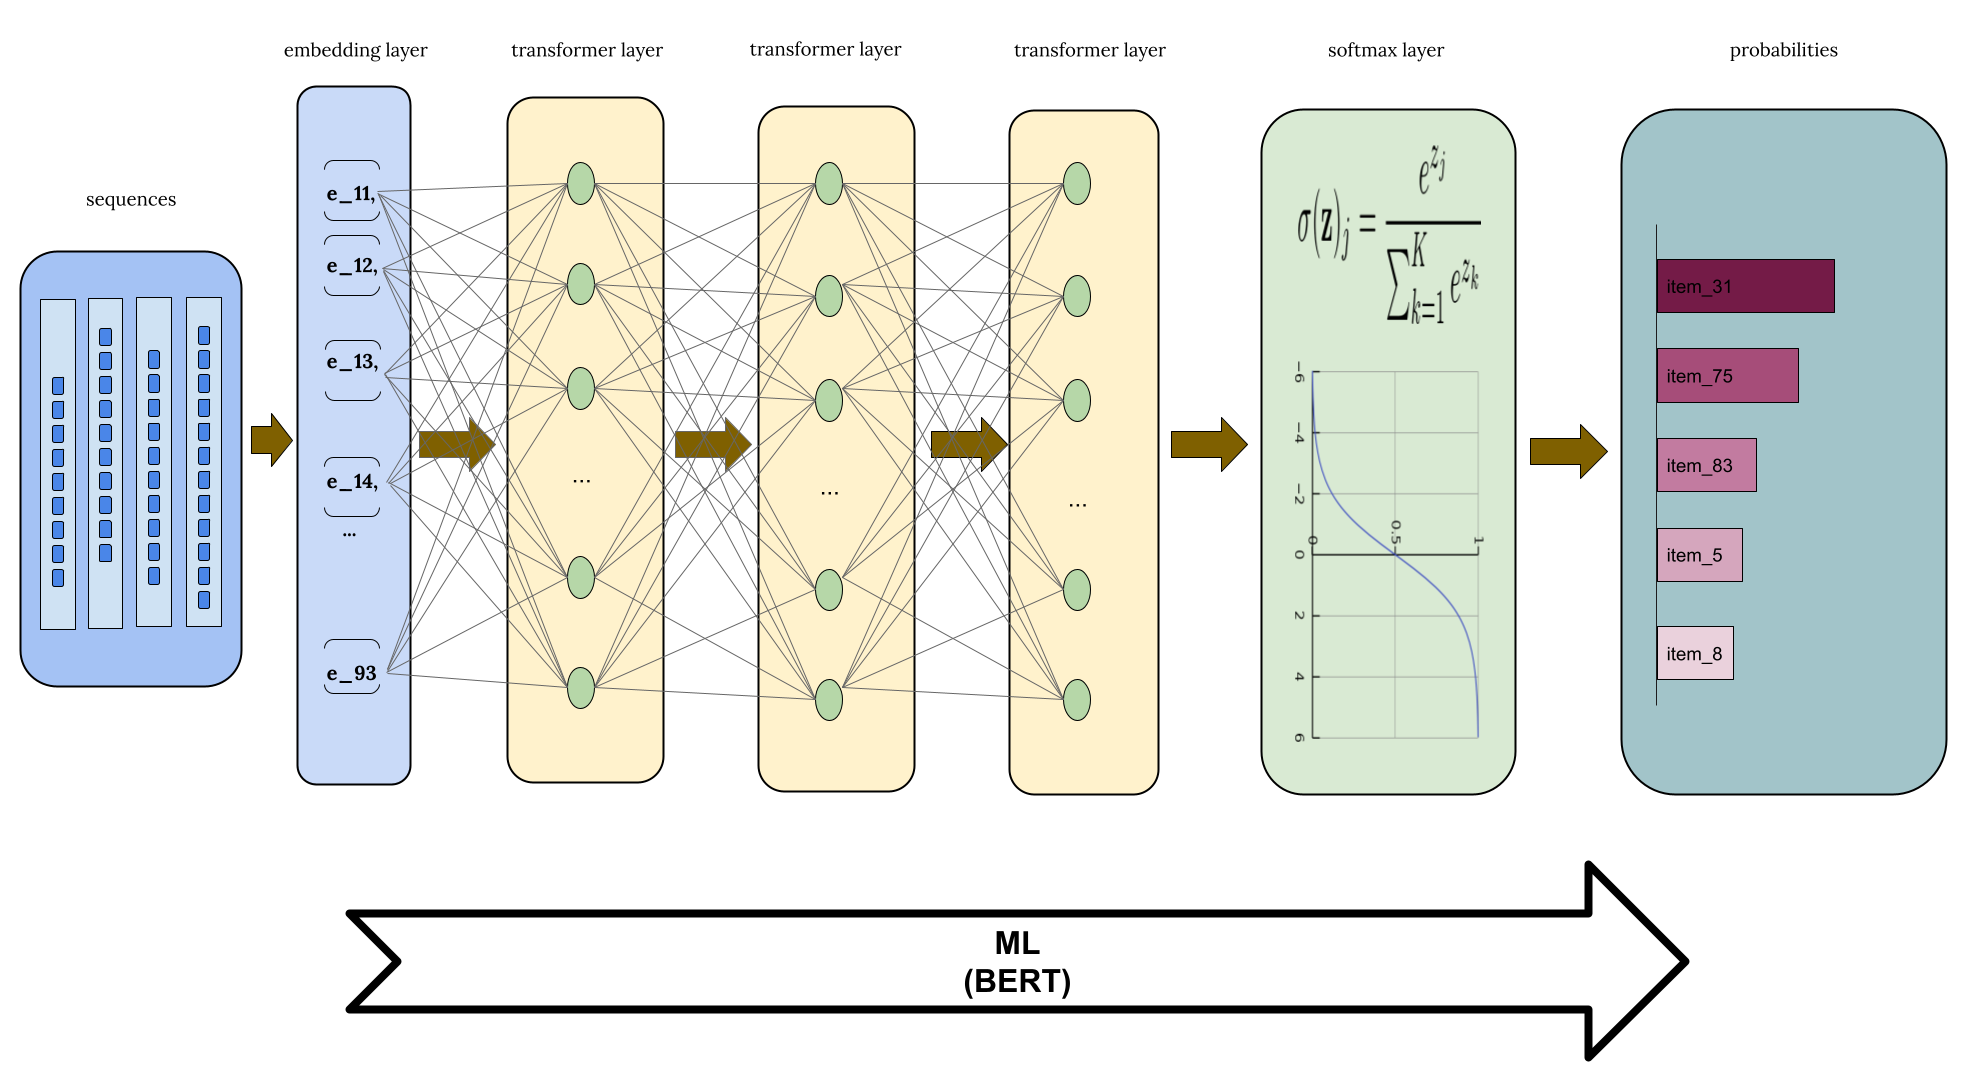
\includegraphics[width=1\textwidth]{images/diagrams/ML_path.png}
\caption{Overview of the ML workflow using BERT.}
\label{fig:ml_flow}
\end{figure}

Depicted in Figure~\ref{fig:ml_flow} is a visualization of our ML workflow using BERT. The sequences get parsed to the model using our custom uniform input converter. Then the modified embedding layer turns the items into temporal embeddings, by combining item vectors with positional vectors and timestamp vectors. The embeddings then flow through the adapted transformer layers of BERT. Our transformer layers pay attention to items in active user sessions and learn about sequential patterns using multi-headed attention. The final layer is a softmax output layer that can predict the next item utilizing a probability distribution.

% D.
% "In the first step, the custom tokenizer turns the items into vector embeddings. For each item, the position in the sequence, as well as the timestamp, get encoded. The embeddings then flow through the transformer layers of BERT. In the transformer layers, BERT learns about sequential patterns using multi-headed attention. The final layer is a softmax output layer that can predict the next item utilizing a probability distribution."
% You're presenting out-of-the-box BERT here, not presenting how we use BERT specifically, right?
% 
% Like
% i) how do we extend BERT to be time-aware?
% ii) how do we make BERT dynamic and able to process data in batches?
% iii) what hyper-parameters from BERT do we pass to meta-learning for automated optimization?
% 
% I.e., all the stuff that's specific to us and that we sold in
% "
% Before we can begin to design our system, we first need to define the requirements. Our goal is to capture data in a fully temporally aware manner and with organic controls. We specify the following requirements:

% \begin{enumerate}
%     \item \emph{Integration of Temporal Patterns} Our system should be able to encode timestamp information from the data.
    
%     \item \emph{Online Training} Our system should adapt to new data in real-time. 
    
%     \item \emph{Meta optimization} Our system should hybridize the different models with organic controls for optimal performance. 
% \end{enumerate}
% "
% that's the angle in which we should be presenting our tools first and foremost, and not a general teaching angle.
% Or we didn't deliver the novel items we sell in the contributions :sweatgrin:, but then it's a different story. Then the whole thesis would only be a review with some re-installation of a few things in the manner of a tutorial. But that wasn't by understanding. Anyway, we should try to be be coherent.

%
% D.
% same feeling when reading the text from "
% \subsection{Model-Based Flow}"
% Man. Less time reviewing everything on earth and more time selling our specificity is usually a good deal. 

% D.
% Also, we've been significantly extending BERT as well as the other two if I am not mistaken. Where do we sell these extensions?
% In background, we're supposed to present vanilla, as things were before we came in, so our extensions shouldn't be there.
% 

\subsection{Model-Based Flow}
Next, we will present our model-based workflow. It is based on a Markov-chain model, which we have enhanced with various extensions. Similar to our BERT model, we use our redesigned uniform input converter to be able to parse a large variety of datasets.

We designed a parallelization computation unit that allows efficient online training in real-time. Although information flows through the layers sequentially, we can compute sequences that don't contain overlapping items separately. Consequently, we create several Markov chains that contain distinct states. New sequences get filtered and passed on to the relevant chain. The model automatically creates new states when unknown items appear and deletes them when items become irrelevant. For efficient resource allocation or to save space, the model can prune states based on the workload. We introduce a notion of importance tracking by summarizing states of important items. New sequences are batched into windows of variable sizes and trained in parallel.

The hyperparameter optimization happens in our custom meta-learning unit. We need to optimize the degree of parallelization, the batch size, and the number of hidden dimensions. 


\begin{figure}[htbp]
\centering
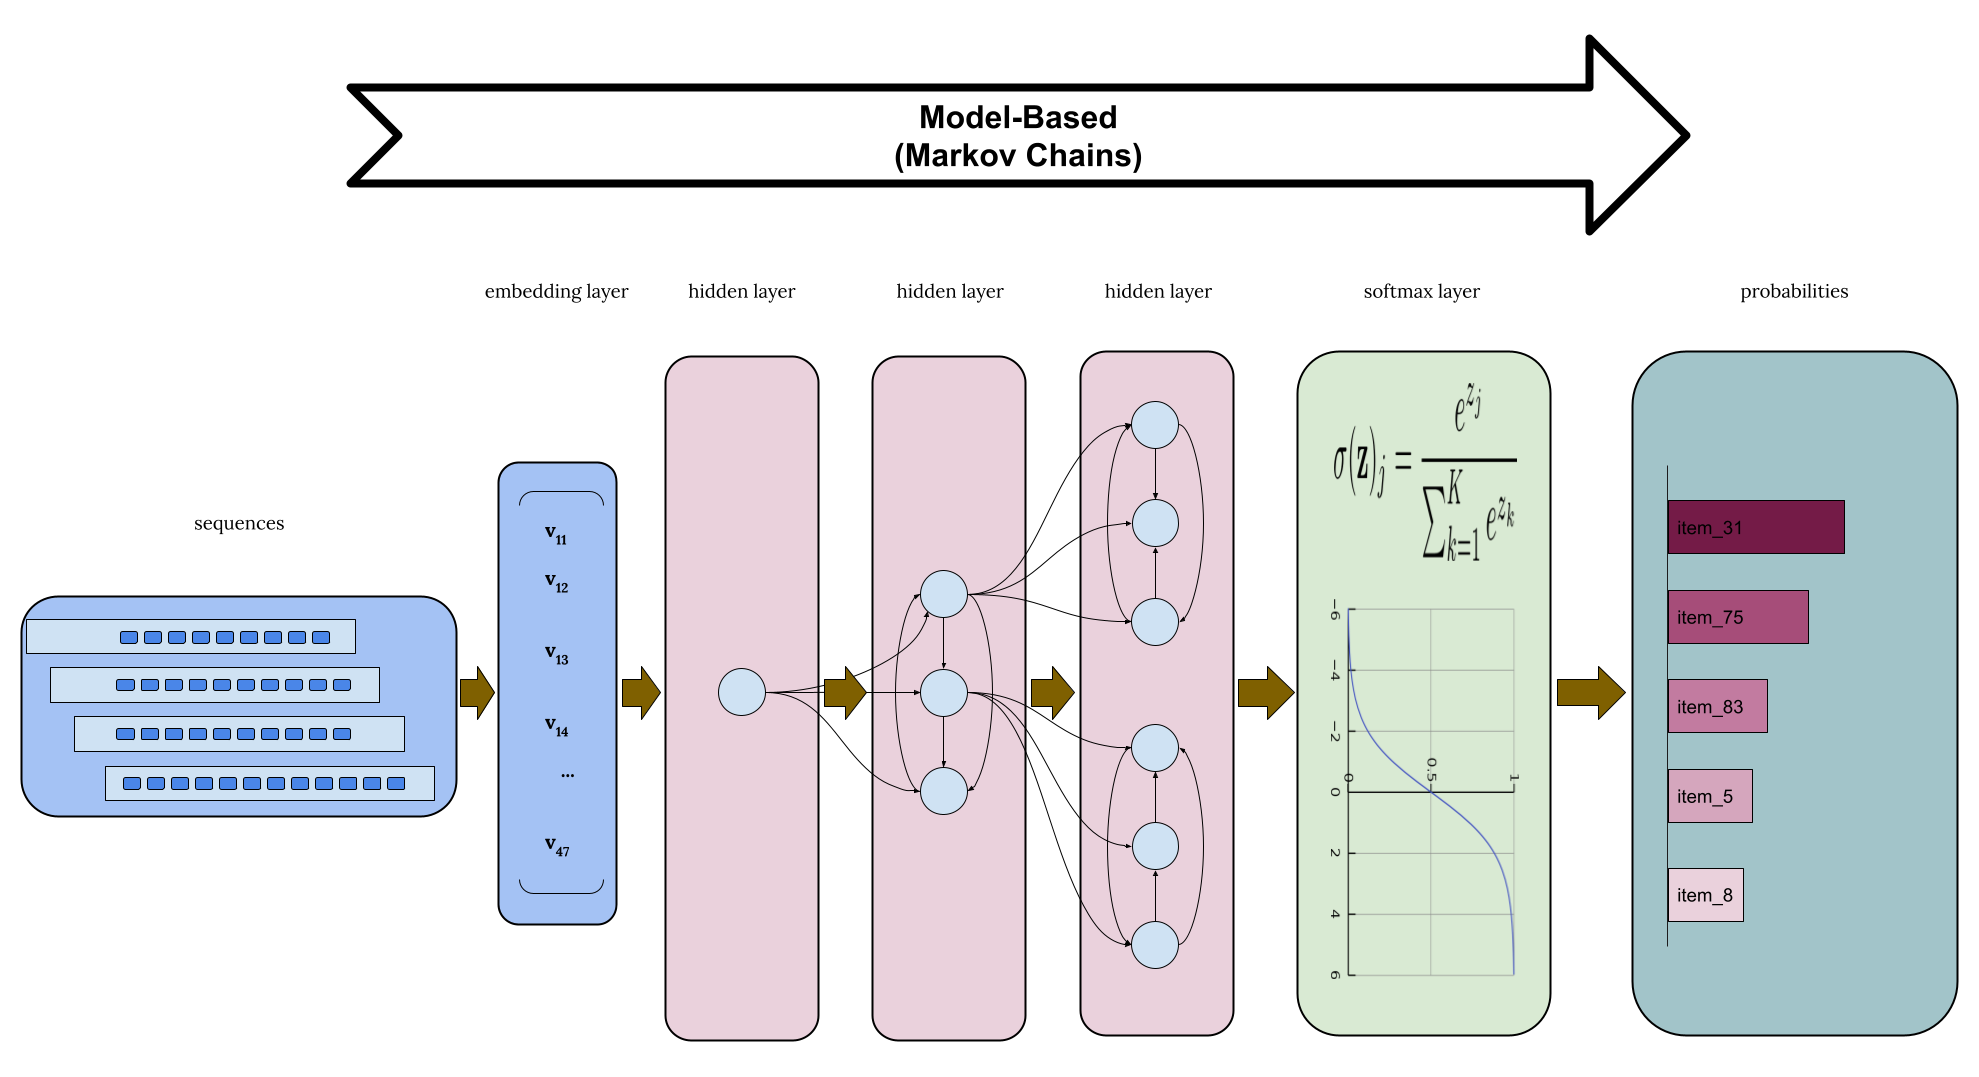
\includegraphics[width=1\textwidth]{images/diagrams/model_based_path.png}
\caption{Overview of the model-based workflow using Markov chains.}
\label{fig:model_based_flow}
\end{figure}

In Figure~\ref{fig:model_based_flow}, we can see our model-based workflow. The custom universal input converter feeds sequences in batches to the embedding layer. The parallelization unit splits up sequences onto different Markov chains as they flow through the hidden layers. Finally, the softmax output layer produces a probability distribution to determine the next item to recommend. This is done using the transition matrices. 


\subsection{Hybridization}

\begin{figure}[htbp]
\centering
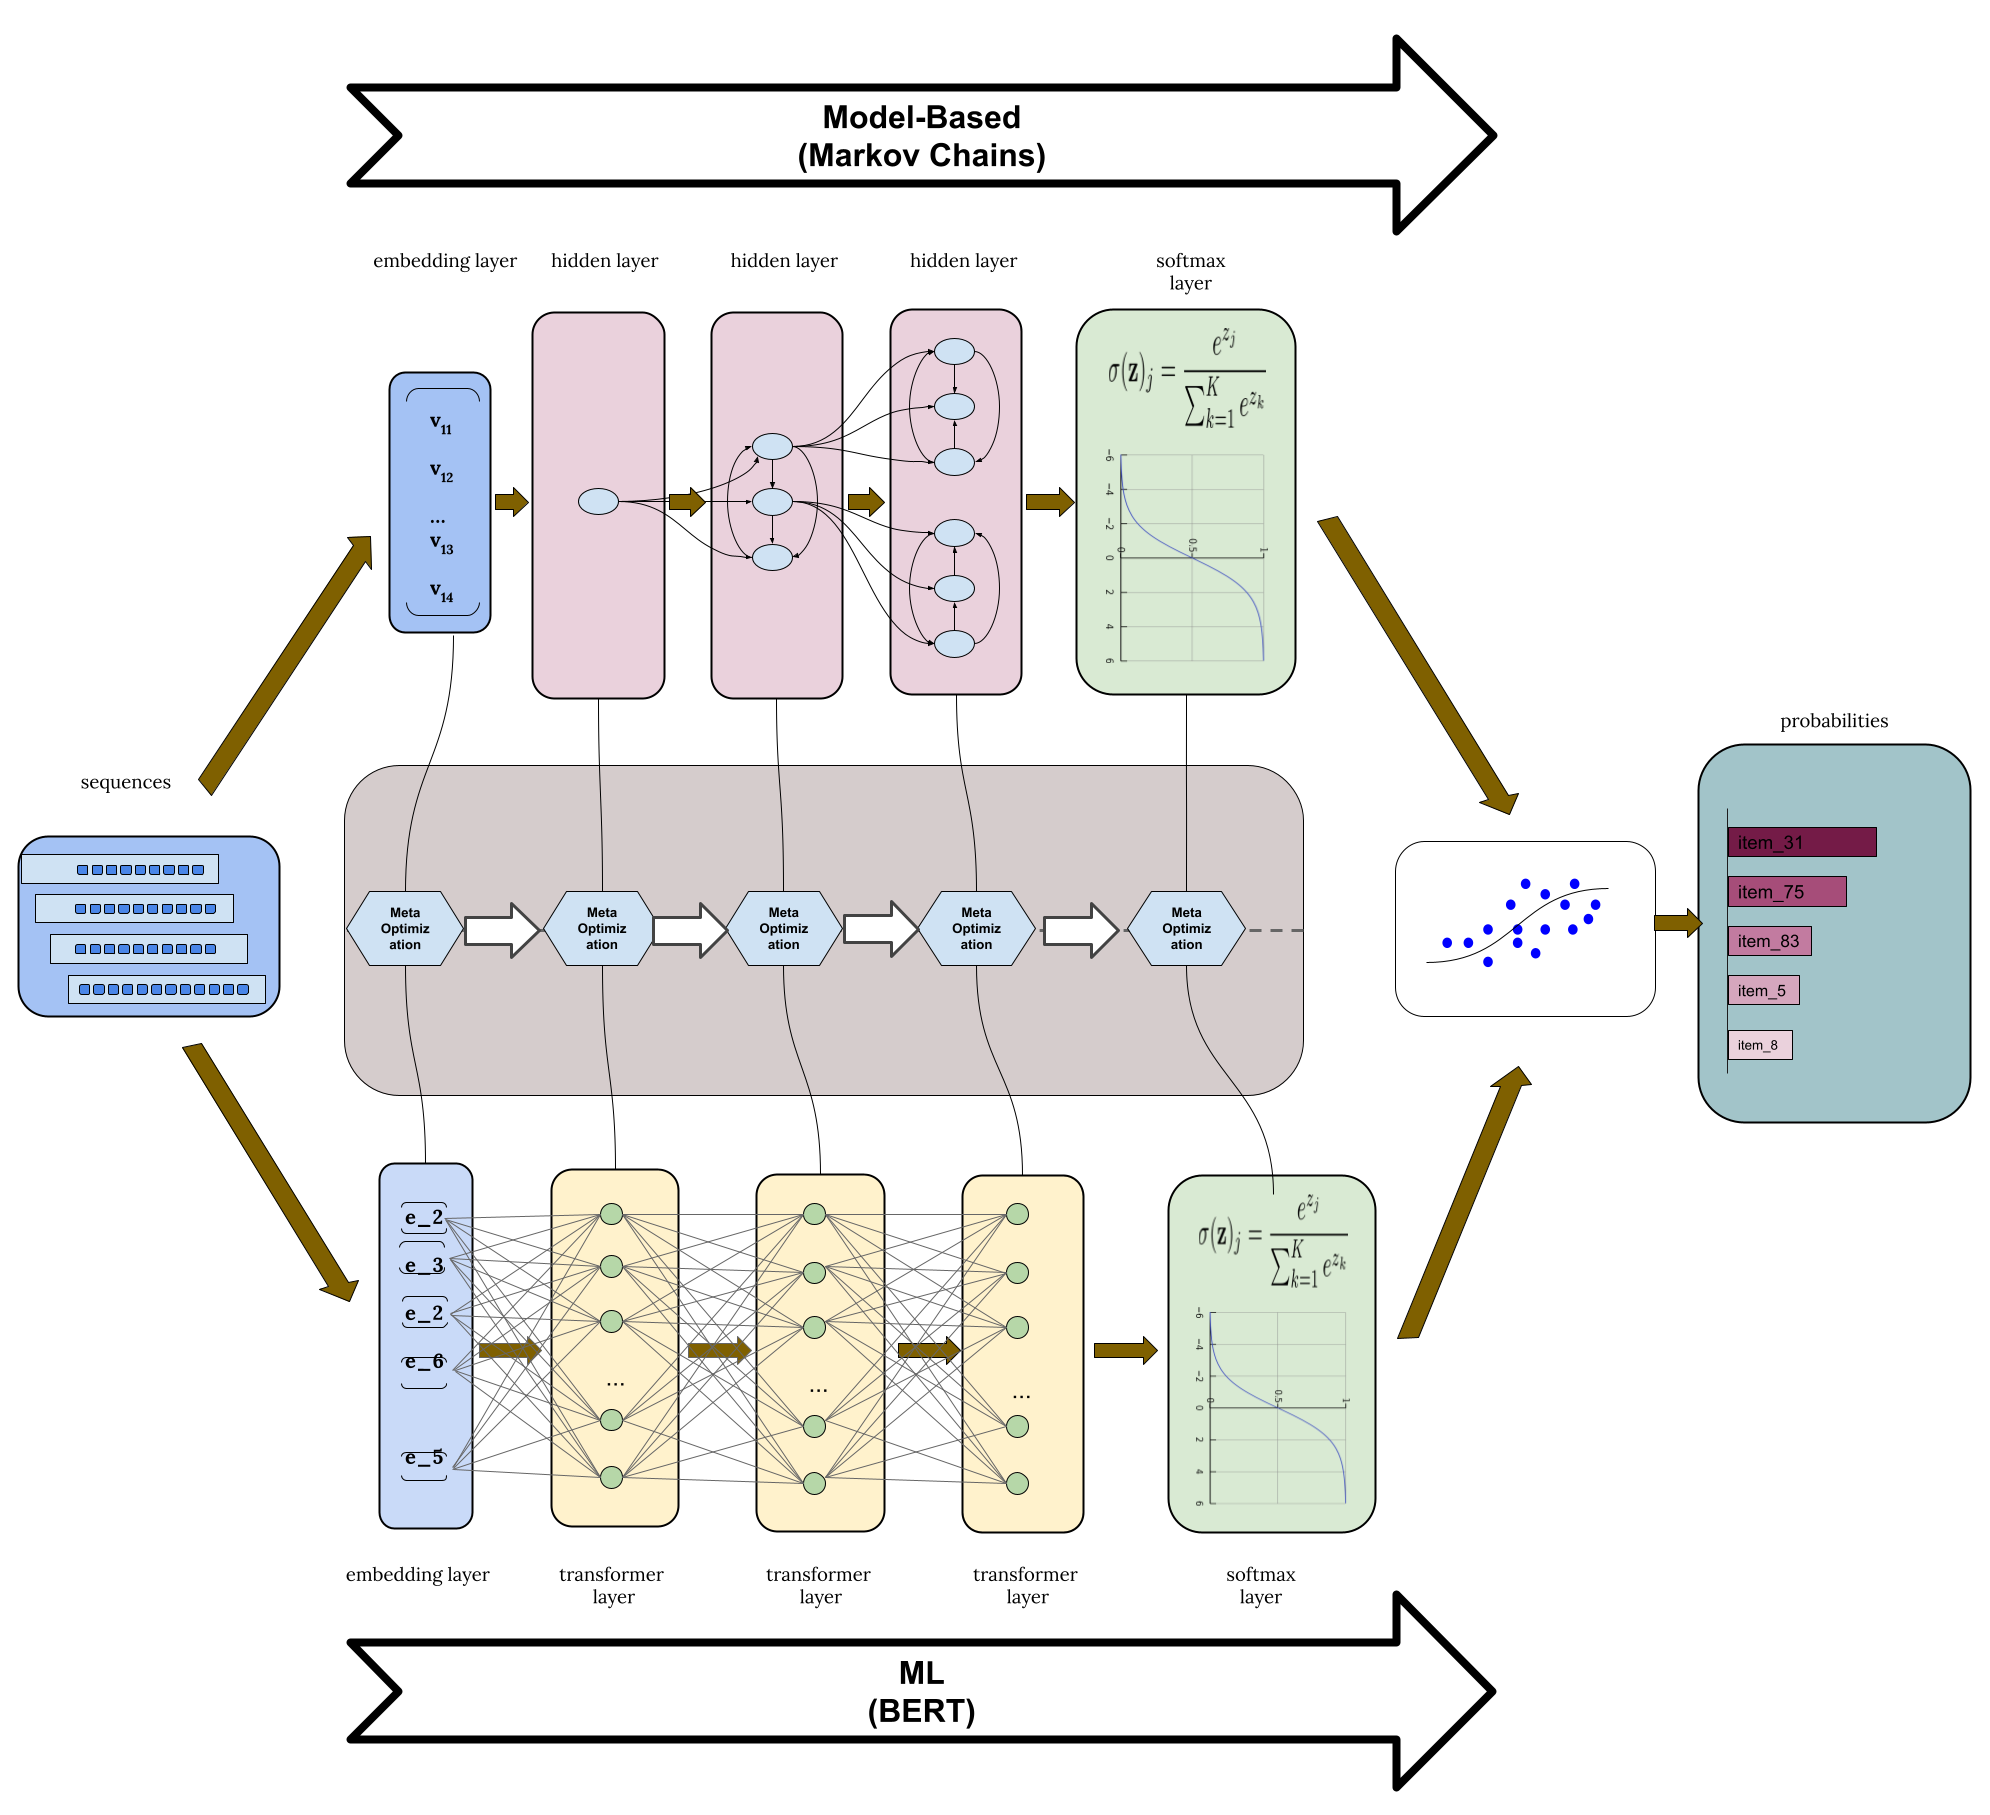
\includegraphics[width=1\textwidth]{images/diagrams/hybrid_path.png}
\caption{Overview of our hybridization workflow}
\label{fig:hybrid_flow}
\end{figure}

We follow a stacking-hybrid approach to combine our models. It is a state-of-the-art technique for hybridization used by many top-performing models~\cite{geron2019hands,pavlyshenko2018using,sikora2015modified,dvzeroski2004combining}. In our implementation of stacking, we aggregate the outputs of the different models for optimal performance as follows~\cite{sagi2018ensemble}:

\begin{equation}
\setlength{\jot}{25pt}
    \begin{aligned}
        \hat{y}=\text{argmax}(\varphi (x_i)) \quad\text{where}\quad \varphi(x_i)= \sum\limits_{m=1}^M w_m*f_m(x_i)
    \end{aligned}
    \label{equation:weighted_avg}
\end{equation}

In Equation~\ref{equation:weighted_avg} we sum up the output probabilities $f_m$ of every model $m\in M$. The item to recommend is based on the highest value in the total vector. Different weights $w_m\in[0,1]$ can be assigned to the models. The goal is to optimize the weights to maximize the accuracy of the output $\hat{y}$. We employ a sophisticated approach to fit the output predictions together with the help of regression. The outputs of the models become meta-features and the weights are the ensemble parameters of a regression function. Our hybridization logic optimizes the hyperparameters of our models. Hyperparameters include the regularization terms for our regression function, learning rates, and dropout rates. The hybrid ratio adapts the weighting of models based on global prediction accuracy. Additionally, the system constantly monitors the accuracy and can reset or retrain individual models dynamically if needed.

The process is depicted in Figure~\ref{fig:hybrid_flow}. As information flows through our hybrid system, the hybridization logic constantly monitors and adapts the hyperparameters based on the available resources and for optimal performance.